\documentclass[fleqn,10pt]{wlscirep}
\usepackage[utf8]{inputenc}
\usepackage[T1]{fontenc}
\usepackage[demo]{graphicx}
\usepackage{caption}
\usepackage{subcaption}
\usepackage{hyperref}
\hypersetup{
    colorlinks=true,
    linkcolor=blue,
    filecolor=magenta,      
    urlcolor=cyan,
}
\usepackage{amsmath} % or simply amstext
\newcommand{\angstrom}{\text{\normalfont\AA}}

\title{A novel nucleoside-enzyme pair for stringent cell-specific metabolic labeling of RNA}

\author[1]{Sarah Nainar}
\author[1]{Bonnie Cuthbert}
\author[1]{Nathan M. Lim}
\author[1]{David L. Mobley}
\author[1]{Celia Goulding}
\author[1, *]{Robert Spitale}
\affil[1]{Department of Pharmaceutical Sciences, University of California---Irvine, Irvine, California 92697, United States}

\affil[*]{rspitale@uci.edu}

\begin{document}

\flushbottom
\maketitle
\tableofcontents

\section{Computational Methods}
The starting structure used for the molecular dynamics (MD) simulations was taken from the crystal structure of human uridine-cytidine kinase 2 complex with the cytidine substrate (PDBID: 1UEJ).
In this study four different MD simulations were carried out, using two different binding modes for each of the respective ligands 2AZU and 2AZC.
Here, we differentiate between the two binding modes by the orientation of the sugar group on the molecule; whereby the "canonnical" binding mode refers to the same orientation of the sugar as found in the crystal structure and the "flipped" binding mode being the opposite.
A total of 500ns of MD simulation time was conducted for each binding mode by running 5 simulations for each binding mode, where each copy of the simulation began from the same protein structure.
The metastable binding modes sampled during our MD simulations were defined by constructing a Markov State Model (MSM) from our pool of MD simulation data and clustering with perron-cluster cluster analysis (PCCA).
We then compared these metastable binding modes with experimental crystal structures for 2AZU and 2AZC by computing the root-mean-square deviation between the ligand heavy atoms.
Our simulation results, along with the x-ray crystal structures, support the hypothesis that the ligands must adopt the "flipped" binding mode for catalytic turnover. 

\subsection{Setup}
\subsubsection{MD simulation parameters}
All simulations in this study were conducted using OpenMM v7.1.1 \cite{openmm} at T=300K and P=1atm.
Here, we use timesteps of 4fs by employing the hydrogen mass repartitioning scheme \cite{hmr}. 
This scheme allows us to take larger timesteps by slowing down the fastest motions (i.e. hydrogen bond stretching) by constraining the bond length between hydrogens and their connected heavy atoms and reallocating mass from the connected heavy atom to the hydrogens.
The protein-ligand systems were placed in a periodic box with explicit TIP3P water molecules using a 10A solvent padding distance and counter ions (NaCl) were added using a concentration of 150mM.
A 10A cut-off distance was used for the particle-mesh Ewald method \cite{}.
Protein atoms were parameterized using the amber99sbildn forcefields \cite{} and ligands were parameterized using GAFF2 \cite{} in which atomic charges were assigned using the AM1-BCC charge model \cite{}

\subsubsection{Protein preparation for MD simulations}
To prepare the protein system for MD simulations, we used PDBFixer \cite{pdbfixer} to model in missing residues, add missing hydrogen atoms, and solvate our system.
Sidechains were protonated in accordance with the pH=8.0 environment \cite{tanaka et. al 4} of the enzyme assay experiments.
With the cytidine molecule bound, we energy minimized the protein-ligand complex for a maximum of 30,000 steps and followed with the equilibration protocol as follows.
The relaxation protocol occurs in four 10 ps stages, whereby a progressively declining restraining force was used to help the protein-ligand system gradually relax.
First we apply a restraining force of 2.0 to the heavy atoms of the protein-ligand complex, simulate for 10ps using constant volume (NVT), and follow-up with 10ps at constant pressure (NPT).
Next, we decrease the restraining force to 0.5 and then conduct an NPT simulation for 10ps.
Last, we use a 0.1 restraining force on the alpha-carbons (protein backbone) and the ligand heavy atoms and then NPT simulate for 10ps.

\subsubsection{Docking the nucleoside analogs}
After equilibration of the UCK2-cytidine complex, we applied HYBRID docking \cite{} to dock our nucleoside analogs (2AZU and 2AZC) into the binding site.
HYBRID differs from the standard docking approach such that it will use the co-crystallized ligand as a reference point and attempt to fit the nucleoside analogs within the binidng site by overlaying the docked ligands with the crystallographic ligand.
From HYBRID docking, we generated up to 50 different conformers for each ligand and then followed the same equilibriation protocol described previously.
After visual inspection, we found that the conformers tended to converge into two groups: 1 conformer which resembled the "cannonical" binding mode and another which had the sugar group "flipped".
We then selected 1 conformer from each representative group and carried these forward for our production NPT 100ns MD simulations (no restraints).

\subsection{Analysis}

% \begin{figure}[!ht]
%   \begin{subfigure}{0.5\textwidth}
%     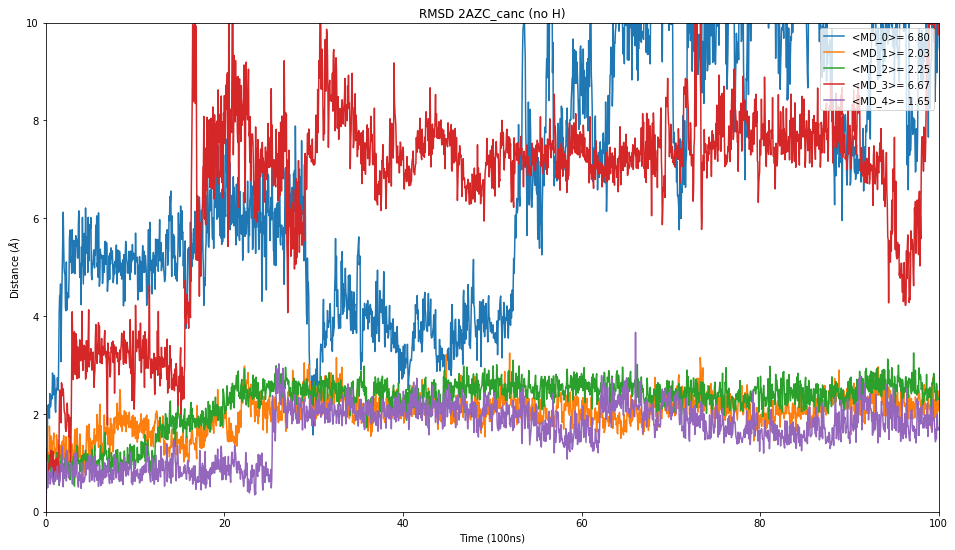
\includegraphics[width=0.95\linewidth, height=5cm]{2AZC_canc/2AZC_canc-rmsd_full} 
%     \caption{2AZC_{canc}-rmsd_full}
%     \label{fig:2AZC_canc-rmsd_full}
%   \end{subfigure}
%   \begin{subfigure}{0.5\textwidth}
%     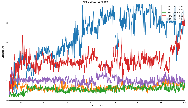
\includegraphics[width=0.95\linewidth, height=5cm]{2AZC_canc/2AZC_canc-rmsd_trim}
%     \caption{2AZC_{canc}-rmsd_trim}
%     \label{fig:2AZC_canc-rmsd_trim}
%   \end{subfigure}
% \caption{Caption for this figure with two images}
% \label{fig:2AZC_canc-rmsd}
% \end{figure}

\href{https://github.com/nathanmlim/Spitale/blob/master/manual_md/notebooks/RMSD-calculations.ipynb}{RMSD-Calculation Jupyter Notebook}

For each nuceloside analog (2AZC and 2AZU), we ran five 100ns MD simulations for each of the two binding modes (cannonical and flipped).
They are denoted as $2AZC_{canc}$, $2AZC_{flip}$, $2AZU_{canc}$, and $2AZU_{flip}$.
Collectively, over the course of the 100ns of simulation time, the root-mean-square deviation (RMSD) for the ligand atoms began to stabilize after 25ns Fig.\ref{fig:2AZC_canc-rmsd_full}.
Thus, we discard trajectory frames from 0-25ns as additional equilibration time and only perform further analysis from the 25ns-100ns time frame Fig.\ref{fig:2AZC_canc-rmsd_trim}.
The RMSD is calculated by:
\begin{equation}
    RMSD = \sqrt{ \frac{1}{n} \sum^{n}_{i=1}{d_{i}^{2}}}
\end{equation}
where $d_{i}$ represents the distance between the $n$ atom pairs.
For construction of our Markov State models (MSM) we use the PyEMMA v2.5.5 \cite{} toolkit.
For residue contact analysis we use the MDTraj v1.9.1 \cite{} toolkit.

\subsubsection{Defining the metastable binding modes}

\begin{figure}[!ht]
\centering
\begin{subfigure}{.5\textwidth}
  \centering
  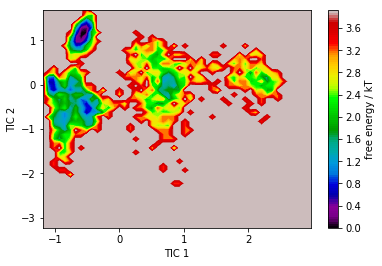
\includegraphics[width=.9\linewidth]{2AZC_canc/2AZC_canc-tica.png}
  \caption{2AZC_{canc}-pcca}
  \label{fig:2AZC_canc-tica}
\end{subfigure}%
\begin{subfigure}{.5\textwidth}
  \centering
  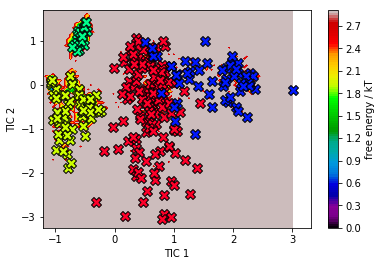
\includegraphics[width=.9\linewidth]{2AZC_canc/2AZC_canc-pcca.png}
  \caption{2AZC_{canc}-pcca}
  \label{fig:2AZC_canc-pcca}
\end{subfigure}
\caption{Caption for this figure with two images}
\label{fig:2AZC_canc-cluster}
\end{figure}

In order to define our metastable binding modes and visualize their structures, we construct a Markov State model (MSM) \cite{} from our five separate MD simulations.
Our features for constructing the MSMs consists of the distance between the closest heavy atoms on the ligand and the following 9 residues: ASP62, PHE83, ASP84, TYR112, PHE114, HIS117, ILE137, ARG166, and ARG176.
These residues were selected as they have been noted in the literature to play important roles in binding \cite{tanaka}.
From this feature space, we apply time-lagged independent component analysis (TICA) using a lagtime of 1ns.
TICA transforms our 9 dimensional feature space to a new set of reaction coordinates which maximizes the autocorrelation of the transformed coordinates \cite{}.
In other words, TICA allows us to extract the slow order parameters and project them into a lower dimensional space; here, we use the first two TICA coordinates (Fig. \ref{fig:2AZC_canc-tica}).
Then, we apply k-means clustering to discretize our trajectory frames into discrete microstate and project them into TICA space (denoted by the individual X).
Following, we use perron-cluster cluster analysis (PCCA) \cite{} to assign each microstate to a metastable macrostate (denoted by color in Fig.\ref{fig:2AZC_canc-pcca}).
From each of our assigned macrostates, we randomly sample 100 frames and then visualize the frame which minimizes the RMSD to the crystallographic ligand.

\subsubsection{Distance to key residues}

\begin{figure}[!ht]
\centering
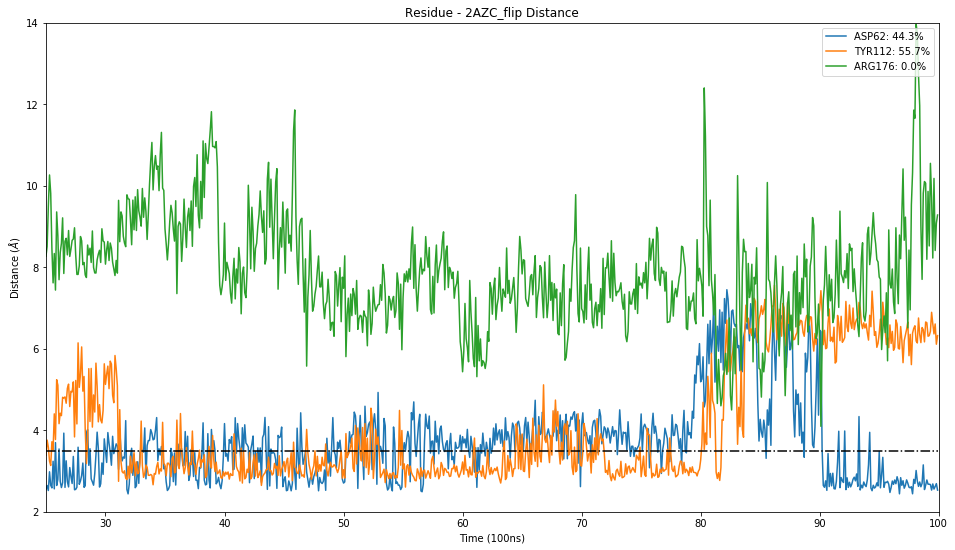
\includegraphics[width=\linewidth]{2AZC_flip/2AZC_flip-distance.png}
\caption{2AZC_{flip}-distance}
\label{fig:2AZC_flip-distance}
\end{figure}

\href{https://github.com/nathanmlim/Spitale/blob/master/manual_md/notebooks/contact-distance.ipynb}{Contact-Distance Jupyter Notebook}

Using the `compute contacts' tool from MDTraj, we compute the distance between the closest heavy atoms in the ligand and 3 residues: ASP62, TYR112, and ARG176 (Fig.\ref{fig:2AZC_flip-distance}).
These residues were chosen in particular as ASP62 is known to be the catalytic reisude, while TYR112 and ARG176 are believed to play a key role in substrate specificity between uridine and cytidine.
Here, we calculate the frequency in which the distance between the ligand and the residues are less than or equal to 3.5A, which we define as the minimum distance needed to form an interactive bond.

\subsubsection{Hydrogen Bond Contacts}

\begin{figure}[!ht]
\centering
\begin{subfigure}{.5\textwidth}
  \centering
  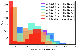
\includegraphics[width=.95\linewidth]{2AZC_flip/2AZC_flip-baker}
  \caption{2AZC_{flip}-baker}
  \label{fig:2AZC_flip-baker}
\end{subfigure}%
\begin{subfigure}{.5\textwidth}
  \centering
  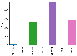
\includegraphics[width=.95\linewidth]{2AZC_flip/2AZC_flip-wernet}
\caption{2AZC_{flip}-wernet}
\label{fig:2AZC_flip-wernet}
\end{subfigure}
\end{figure}

\href{https://github.com/nathanmlim/Spitale/blob/master/manual_md/notebooks/Hbonds.ipynb}{Hbonds Jupyter Notebook.}

We compute the frequency of hydrogen bond contacts between the ligands and surround residues using two methods from MDTraj: the Bakker-Hubbard \cite{} and the Wernet-Nilsson methods \cite{}.
The donors considered by these methods are `NH' and `OH' and the acceptors considered are `O' and `N' 
Fig.\ref{fig:2AZC_flip-baker} shows the Bakker-Hubbard method which identifies hydrogen bonds based on a cutoff distance $d<2.5\angstrom$ and an angle $\theta>120$.
Fig.\ref{fig:2AZC_flip-wernet} shows the Wernet-Nilsson method employs a different method where distance cutoff depends on the angle.
The criterion employed is 
\begin{equation}
r_{DA}<3.3\angstrom - 0.00044 \times \delta{H_{DA}} \times \delta{H_{DA}}
\end{equation} where $r_{DA}$ is the distance between donor and acceptor heavy atoms, and $\delta{H_{DA}}$ is the angle made by the hydrogen atom, donor, and acceptor atoms, measured in degrees.
With the Wernet-Nilsson method, we only count hydrogen bond contacts if the are formed at least $5\%$ of the simulation time.


\subsubsection{Comparisons to Xtal}
To compare the metastable binding modes from our MD simulations with experimental x-ray crystal structures, we first align the two structures using the protein backbone.
Particularly, we align by the protein backbone using residues 19 to 229 but exclude residues 48 to 52 as these were missing in the x-ray crystal structure.
Once aligned by the protein backbone, we then compute the RMSD between the ligand heavy atoms using our defined metastable binding modes from our PCCA analysis.
The x-ray crystal structure of 2AZC represents the system in it's post-catalytic state and has a phosphate group attached, thus we exclude the phosphate group from our RMSD calculations as our simulations represent the pre-catalytic state.
The x-ray crystal structure of 2AZU represents the system in it's pre-catalytic state and has no additional phosphate group, so no atoms were excluded from the RMSD calculation.


\section{Results}

\subsection{Binding Mode Stability}

\begin{figure}[!ht]
\centering
   \begin{subfigure}{.45\textwidth}
     \centering
     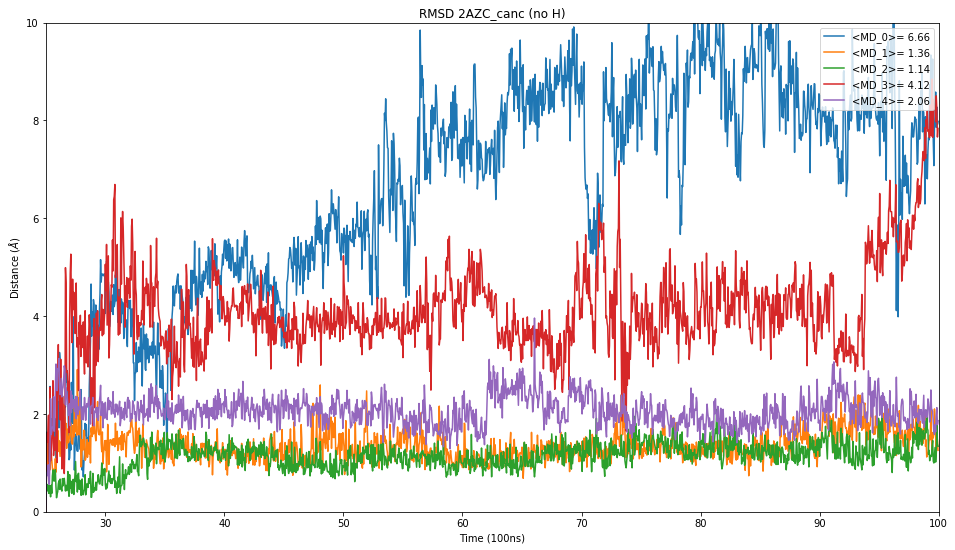
\includegraphics[width=.95\linewidth]{2AZC_canc/2AZC_canc-rmsd-trim.png}
     \caption{2AZC_{canc}-rmsd_trim}
     \label{fig:2AZC_canc-rmsd_trim}
   \end{subfigure}
   \begin{subfigure}{.45\textwidth}
     \centering
     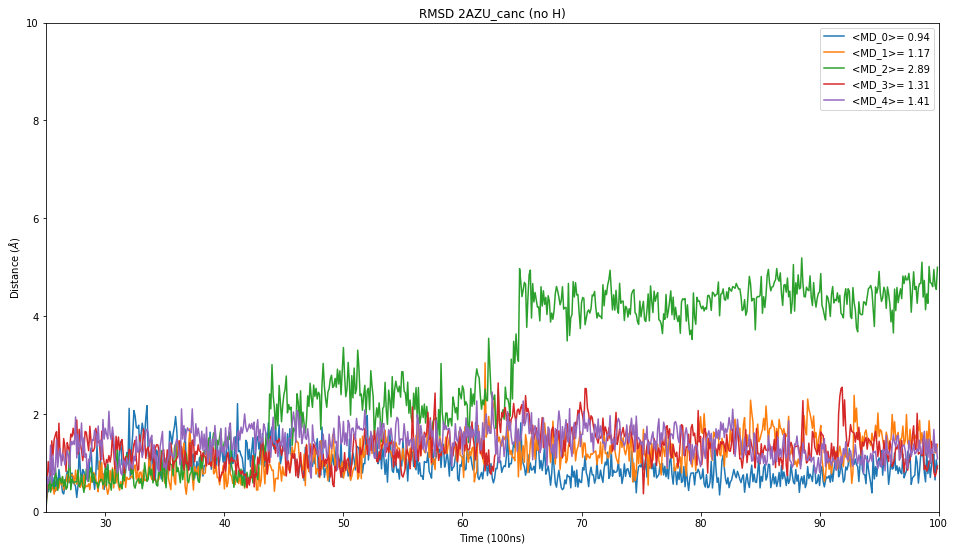
\includegraphics[width=.95\linewidth]{2AZU_canc/2AZU_canc-rmsd-trim.png}
     \caption{2AZU_{canc}-rmsd_trim}
     \label{fig:2AZU_canc-rmsd_trim}
   \end{subfigure}
   \\
   \begin{subfigure}{.45\textwidth}
     \centering
     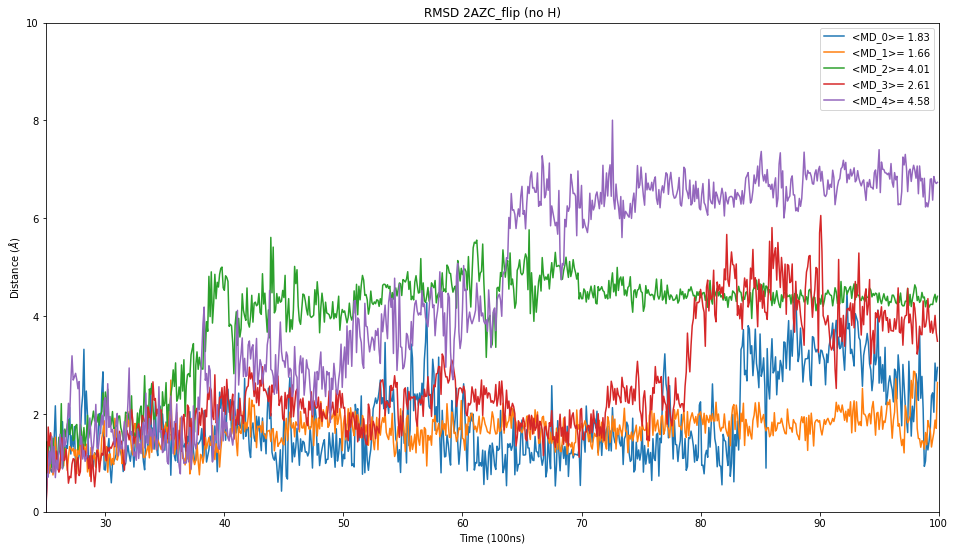
\includegraphics[width=.95\linewidth]{2AZC_flip/2AZC_flip-rmsd-trim.png}
     \caption{2AZC_{flip}-rmsd_trim}
     \label{fig:2AZC_flip-rmsd_trim}
   \end{subfigure}
    \begin{subfigure}{.45\textwidth}
     \centering
     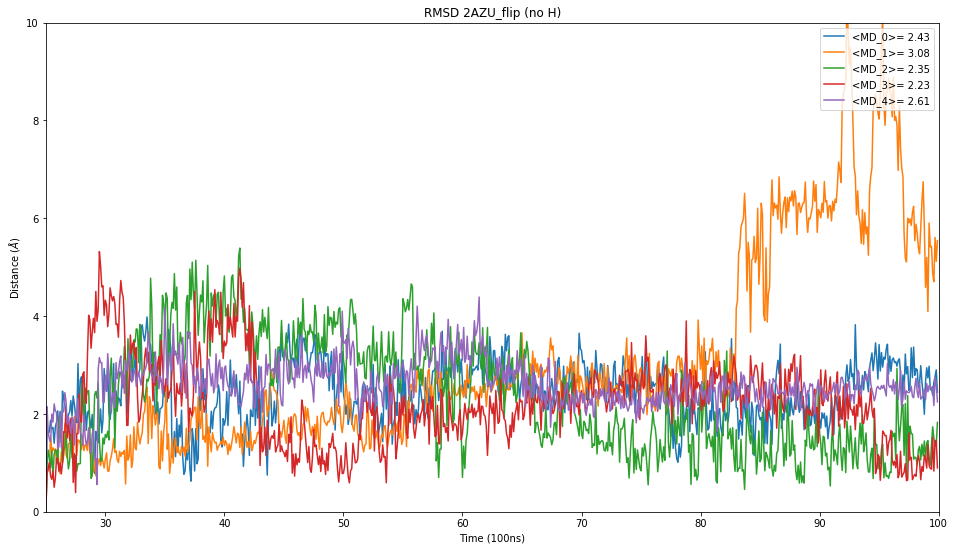
\includegraphics[width=.95\linewidth]{2AZU_flip/2AZU_flip-rmsd-trim.png}
     \caption{2AZU_{flip}-rmsd_trim}
     \label{fig:2AZU_flip-rmsd_trim}
   \end{subfigure}
\end{figure}  

\begin{table}[!ht]
\caption{Calculated RMSDs for ligand heavy atoms from 25-100ns MD simulations}
\label{table:rmsd}
\begin{tabular}{|l|l|l|l|l|l|l|l|}
\hline
                    & RMSD & RMSD & RMSD & RMSD & RMSD & \textbf{AVG}  & SEM           \\ \hline
\textbf{2AZC\_canc} & 6.66 & 1.36 & 1.14 & 4.12 & 2.06 & \textbf{3.07} & \textit{1.04} \\ \hline
\textbf{2AZU\_canc} & 0.94 & 1.17 & 2.89 & 1.31 & 1.41 & \textbf{1.54} & \textit{0.35} \\ \hline
\textbf{2AZC\_flip} & 1.83 & 1.66 & 4.01 & 2.61 & 4.58 & \textbf{2.94} & \textit{0.58} \\ \hline
\textbf{2AZU\_flip} & 2.43 & 3.08 & 2.35 & 2.23 & 2.61 & \textbf{2.54} & \textit{0.15} \\ \hline

\end{tabular}
\end{table}

The averages and the standard errors of the mean (SEM) for the RMSD of each ligand binding mode are shown in Fig.\ref{fig:rmsd} and Table\ref{table:rmsd}.
They are $3.07 \frac{+}{-} 1.04$, $1.54 \frac{+}{-} 0.35$, $2.94 \frac{+}{-} 0.58$, and $2.54 \frac{+}{-} 0.15$ for $2AZC_{canc}$, $2AZU_{canc}$, $2AZC_{flip}$, and $2AZU_{flip}$, respectively.

Comparing the RMSD of the cannonical binding modes for 2AZC and 2AZU, we find that the 2AZU ligand to be much more stable than the 2AZC ligand.
In $\frac{2}{5}$ of our MD simulations for $2AZC_{canc}$ (Fig.\ref{fig:2AZC_canc-rmsd_trim}), the ligand comes nearly unbound after 30ns; while for $2AZU_{canc}$ (Fig. \ref{fig:2AZU_canc-rmsd_trim}) the ligand nearly unbinds in only $\frac{1}{5}$ of the simulations.

Prior to running our MD simulations, we had no experimental evidence for the existence of the flipped binding mode.
The flipped binding mode was first discovered after our HYBRID docking approach with our short equilibration protocol.
When comparing $2AZC_{flip}$ and $2AZU_{flip}$, the average RMSD suggests both are about equally stable.
However, this particular binding mode appears to show slightly more instability than the cannonical binding mode with an average RMSD of $2.54$ and $2.94$ for the $2AZC_{flip}$ and $2AZU_{flip}$, respectively.

\subsubsection{Distance to key residues}


\subsubsection*{RMSD calculation to Xtal chains}

\subsection*{Flipped Binding Mode 2AZC vs 2AZU}
\subsubsection*{Distance to key residues ASP62, TYR112, ARG}
\subsubsection*{RMSD calculation to Xtal chains}


\section*{Discussion}
Support hypotheses:

  - Evidence of flipped binding mode
  
  - 2AZC > 2AZU
  
     - Number of HBond contacts
     
     - RMSD for 20 - 100 ns?

Highlight:

  - ASP62 - TYR112 coupling importance for binding

The Discussion should be succinct and must not contain subheadings.



%\bibliography{sample}

%\noindent LaTeX formats citations and references automatically using the bibliography records in your .bib file, which you can edit via the project menu. Use the cite command for an inline citation, e.g.  \cite{Hao:gidmaps:2014}.

%For data citations of datasets uploaded to e.g. \emph{figshare}, please use the \verb|howpublished| option in the bib entry to specify the platform and the link, as in the \verb|Hao:gidmaps:2014| example in the sample bibliography file.

%\section*{Acknowledgements (not compulsory)}

%Acknowledgements should be brief, and should not include thanks to anonymous referees and editors, or effusive comments. Grant or contribution numbers may be acknowledged.

%\section*{Author contributions statement}

%Must include all authors, identified by initials, for example:
%A.A. conceived the experiment(s),  A.A. and B.A. conducted the experiment(s), C.A. and %D.A. analysed the results.  All authors reviewed the manuscript. 

%\section*{Additional information}

%To include, in this order: \textbf{Accession codes} (where applicable); \textbf{Competing interests} (mandatory statement). 

%The corresponding author is responsible for submitting a \href{http://www.nature.com/srep/policies/index.html#competing}{competing interests statement} on behalf of all authors of the paper. This statement must be included in the submitted article file.

%\begin{figure}[ht]
%\centering
%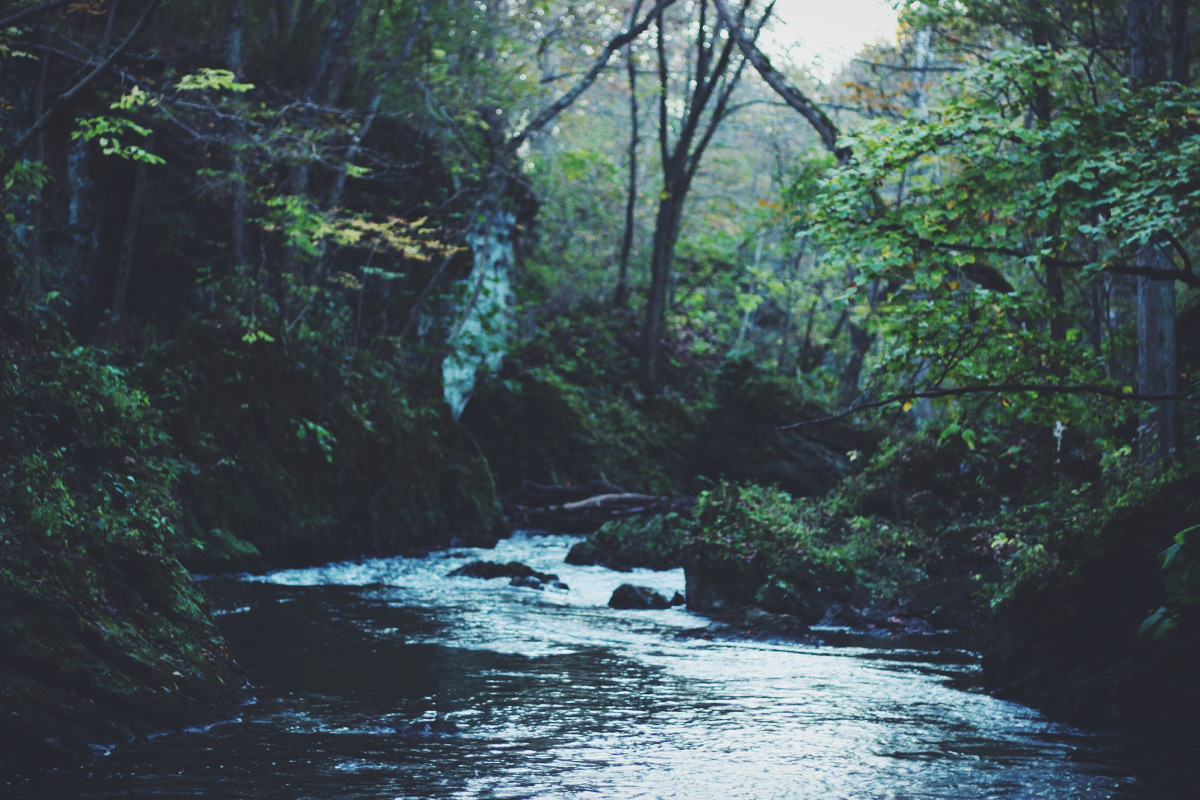
\includegraphics[width=\linewidth]{stream}
%\caption{Legend (350 words max). Example legend text.}
%\label{fig:stream}
%\end{figure}

%\begin{table}[ht]
%\centering
%\begin{tabular}{|l|l|l|}
%\hline
%Condition & n & p \\
%\hline
%A & 5 & 0.1 \\
%\hline
%B & 10 & 0.01 \\
%\hline
%\end{tabular}
%\caption{\label{tab:example}Legend (350 words max). Example legend text.}
%\end{table}

%Figures and tables can be referenced in LaTeX using the ref command, e.g. Figure \ref{fig:stream} and Table \ref{tab:example}.

\end{document}